\documentclass{beamer}

% Should be documentclass beamer

\mode<presentation>
{
%  \usetheme[hideothersubsections]{PaloAlto}
  \usetheme{metropolis}
  \setbeamercovered{transparent}
}

\usepackage{amsfonts}
\usepackage{amsmath}
\usepackage{amssymb}
\usepackage{color}
\usepackage{tikz}
\usepackage{pgfplots}
\usepackage{listings}
\usepackage{courier}
%\usepackage[utf8]{inputenc}
%\usepackage[russian]{babel}

\lstset{
  numbers=left,
  basicstyle=\ttfamily\footnotesize,
  numberstyle=\tiny\color{gray},
  stepnumber=1,
  numbersep=10pt,
}

\newcommand{\iu}{\ensuremath{\mathrm{i}}}
\newcommand{\bbR}{\mathbb{R}}
\newcommand{\bbC}{\mathbb{C}}
\newcommand{\calV}{\mathcal{V}}
\newcommand{\calW}{\mathcal{W}}
\newcommand{\macheps}{\epsilon_{\mathrm{mach}}}
\newcommand{\matlab}{\textsc{Matlab}}

\newcommand{\ddiag}{\operatorname{diag}}
\newcommand{\fl}{\operatorname{fl}}
\newcommand{\nnz}{\operatorname{nnz}}
\newcommand{\tr}{\operatorname{tr}}
\renewcommand{\vec}{\operatorname{vec}}

\newcommand{\vertiii}[1]{{\left\vert\kern-0.25ex\left\vert\kern-0.25ex\left\vert #1
    \right\vert\kern-0.25ex\right\vert\kern-0.25ex\right\vert}}
\newcommand{\ip}[2]{\langle #1, #2 \rangle}
\newcommand{\ipx}[2]{\left\langle #1, #2 \right\rangle}
\newcommand{\order}[1]{O( #1 )}

\newcommand{\kron}{\otimes}


\newcommand{\hdr}[2]{
  \title[CS 5220, Fall 2017]{CS 5220: #2}
  \author{David Bindel}
  \date{#1}
}


\hdr{2017-09-12}{Locality and parallelism in simulations I}


\begin{document}

\begin{frame}
  \titlepage
\end{frame}


\begin{frame}
  \frametitle{Parallelism and locality}

  \begin{itemize}
  \item Real world exhibits {\em parallelism} and {\em locality}
    \begin{itemize}
    \item Particles, people, etc function independently
    \item Nearby objects interact more strongly than distant ones
    \item Can often simplify dependence on distant objects
    \end{itemize}
  \item Can get more parallelism / locality through model
    \begin{itemize}
    \item Limited range of dependency between adjacent time steps
    \item Can neglect or approximate far-field effects
    \end{itemize}
  \item Often get parallism at multiple levels
    \begin{itemize}
    \item Hierarchical circuit simulation
    \item Interacting models for climate
    \item Parallelizing individual experiments in MC or optimization
    \end{itemize}
  \end{itemize}
\end{frame}


\begin{frame}
  \frametitle{Basic styles of simulation}

  \begin{itemize}
  \item Discrete event systems (continuous or discrete time)
    \begin{itemize}
    \item Game of life, logic-level circuit simulation
    \item Network simulation
    \end{itemize}
  \item Particle systems
    \begin{itemize}
    \item Billiards, electrons, galaxies, ...
    \item Ants, cars, ...?
    \end{itemize}
  \item Lumped parameter models (ODEs)
    \begin{itemize}
    \item Circuits (SPICE), structures, chemical kinetics
    \end{itemize}
  \item Distributed parameter models (PDEs / integral equations)
    \begin{itemize}
    \item Heat, elasticity, electrostatics, ...
    \end{itemize}
  \end{itemize}
  Often more than one type of simulation appropriate. \\
  Sometimes more than one at a time!

\end{frame}


\begin{frame}
  \frametitle{Discrete events}

  Basic setup:
  \begin{itemize}
  \item Finite set of variables, updated via transition function
  \item {\em Synchronous} case: finite state machine
  \item {\em Asynchronous} case: event-driven simulation
  \item Synchronous example: Game of Life
  \end{itemize}

  \vspace{5mm}
  Nice starting point --- no discretization concerns!
\end{frame}


\begin{frame}
  \frametitle{Game of Life}

  \begin{center}
    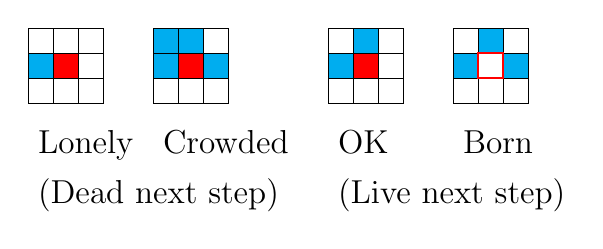
\begin{tikzpicture}[y=-1cm]

% objects at depth 50:
\draw[black] (0.635,0.635) rectangle (1.5875,1.5875);
\path[draw=black,fill=red] (0.9525,0.9525) rectangle (1.27,1.27);
\draw[black] (0.635,0.9525) -- (1.5875,0.9525);
\draw[black] (0.635,1.27) -- (1.5875,1.27);
\draw[black] (0.9525,0.635) -- (0.9525,1.5875);
\draw[black] (1.27,0.635) -- (1.27,1.5875);
\draw[black] (2.2225,0.635) rectangle (3.175,1.5875);
\path[draw=black,fill=red] (2.54,0.9525) rectangle (2.8575,1.27);
\draw[black] (2.2225,0.9525) -- (3.175,0.9525);
\draw[black] (2.2225,1.27) -- (3.175,1.27);
\draw[black] (2.54,0.635) -- (2.54,1.5875);
\draw[black] (2.8575,0.635) -- (2.8575,1.5875);
\draw[black] (4.445,0.635) rectangle (5.3975,1.5875);
\path[draw=black,fill=red] (4.7625,0.9525) rectangle (5.08,1.27);
\draw[black] (4.445,0.9525) -- (5.3975,0.9525);
\draw[black] (4.445,1.27) -- (5.3975,1.27);
\draw[black] (4.7625,0.635) -- (4.7625,1.5875);
\draw[black] (5.08,0.635) -- (5.08,1.5875);
\draw[black] (6.0325,0.635) rectangle (6.985,1.5875);
\draw[black] (6.0325,0.9525) -- (6.985,0.9525);
\draw[black] (6.35,0.635) -- (6.35,1.5875);
\draw[black] (6.35,0.9525) rectangle (6.6675,1.27);
\draw[black] (6.0325,1.27) -- (6.985,1.27);
\draw[black] (6.6675,0.635) -- (6.6675,1.5875);
\path[draw=black,fill=cyan] (2.54,0.9525) rectangle (2.2225,1.27);
\path[draw=black,fill=cyan] (2.8575,0.635) rectangle (2.54,0.9525);
\path[draw=black,fill=cyan] (2.54,0.635) rectangle (2.2225,0.9525);
\path[draw=black,fill=cyan] (3.175,0.9525) rectangle (2.8575,1.27);
\path[draw=black,fill=cyan] (4.7625,0.9525) rectangle (4.445,1.27);
\path[draw=black,fill=cyan] (5.08,0.635) rectangle (4.7625,0.9525);
\path[draw=black,fill=cyan] (6.6675,0.635) rectangle (6.35,0.9525);
\path[draw=black,fill=cyan] (6.35,0.9525) rectangle (6.0325,1.27);
\path[draw=black,fill=cyan] (6.985,0.9525) rectangle (6.6675,1.27);
\path[draw=black,fill=cyan] (0.9525,0.9525) rectangle (0.635,1.27);
\draw[semithick,red] (6.6675,0.9525) rectangle (6.35,1.27);
\path (0.635,2.2225) node[text=black,anchor=base west] {\large{}Lonely};
\path (2.2225,2.2225) node[text=black,anchor=base west] {\large{}Crowded};
\path (4.445,2.2225) node[text=black,anchor=base west] {\large{}OK};
\path (6.0325,2.2225) node[text=black,anchor=base west] {\large{}Born};
\path (0.635,2.8575) node[text=black,anchor=base west] {\large{}(Dead next step)};
\path (4.445,2.8575) node[text=black,anchor=base west] {\large{}(Live next step)};

\end{tikzpicture}%

  \end{center}

  Game of Life (John Conway):
  \begin{enumerate}
  \item Live cell dies with < 2 live neighbors
  \item Live cell dies with > 3 live neighbors
  \item Live cell lives with 2--3 live neighbors
  \item Dead cell becomes live with exactly 3 live neighbors
  \end{enumerate}
\end{frame}

\begin{frame}
  \frametitle{Game of Life}

  \begin{center}
    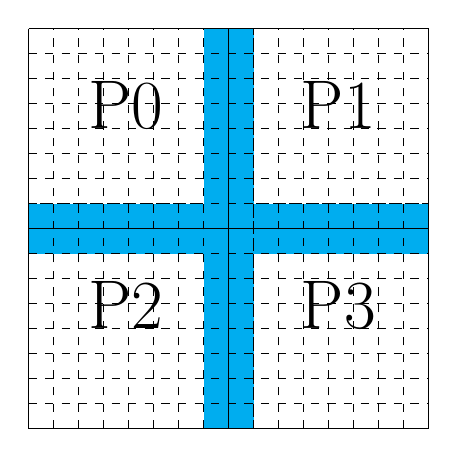
\begin{tikzpicture}[y=-1cm]

% objects at depth 60:
\path[draw=black,fill=cyan,dashed] (1.27,3.4925) rectangle (6.35,4.1275);
\path[draw=black,fill=cyan,dashed] (3.4925,6.35) rectangle (4.1275,1.27);

% objects at depth 50:
\draw[dashed,black] (1.27,4.1275) -- (6.35,4.1275);
\draw[dashed,black] (1.27,4.445) -- (6.35,4.445);
\draw[dashed,black] (1.27,4.7625) -- (6.35,4.7625);
\draw[dashed,black] (1.27,5.08) -- (6.35,5.08);
\draw[dashed,black] (1.27,5.3975) -- (6.35,5.3975);
\draw[dashed,black] (1.27,5.715) -- (6.35,5.715);
\draw[dashed,black] (1.27,6.0325) -- (6.35,6.0325);
\draw[dashed,black] (1.27,3.4925) -- (6.35,3.4925);
\draw[dashed,black] (1.27,3.175) -- (6.35,3.175);
\draw[dashed,black] (1.27,2.8575) -- (6.35,2.8575);
\draw[dashed,black] (1.27,1.905) -- (6.35,1.905);
\draw[dashed,black] (1.27,1.5875) -- (6.35,1.5875);
\draw[dashed,black] (1.5875,6.35) -- (1.5875,1.27);
\draw[dashed,black] (2.54,6.35) -- (2.54,1.27);
\draw[dashed,black] (2.8575,6.35) -- (2.8575,1.27);
\draw[dashed,black] (3.175,6.35) -- (3.175,1.27);
\draw[dashed,black] (3.4925,6.35) -- (3.4925,1.27);
\draw[dashed,black] (4.1275,6.35) -- (4.1275,1.27);
\draw[dashed,black] (4.445,6.35) -- (4.445,1.27);
\draw[dashed,black] (4.7625,6.35) -- (4.7625,1.27);
\draw[dashed,black] (5.08,6.35) -- (5.08,1.27);
\draw[dashed,black] (5.3975,6.35) -- (5.3975,1.27);
\draw[dashed,black] (5.715,6.35) -- (5.715,1.27);
\draw[dashed,black] (6.0325,6.35) -- (6.0325,1.27);
\draw[semithick,black] (6.35,1.27) -- (6.35,6.35);
\draw[semithick,black] (1.27,1.27) -- (6.35,1.27);
\draw[semithick,black] (1.27,1.27) -- (1.27,6.35);
\draw[semithick,black] (1.27,6.35) -- (6.35,6.35);
\draw[semithick,black] (3.81,1.27) -- (3.81,6.35);
\draw[semithick,black] (1.27,3.81) -- (6.35,3.81);
\draw[dashed,black] (1.27,2.54) -- (6.35,2.54);
\draw[dashed,black] (1.905,6.35) -- (1.905,1.27);
\draw[dashed,black] (1.27,2.2225) -- (6.35,2.2225);
\draw[dashed,black] (2.2225,6.35) -- (2.2225,1.27);
\path (1.905,2.54) node[text=black,anchor=base west] {\Huge{}P0};
\path (4.60375,2.54) node[text=black,anchor=base west] {\Huge{}P1};
\path (1.905,5.08) node[text=black,anchor=base west] {\Huge{}P2};
\path (4.60375,5.08) node[text=black,anchor=base west] {\Huge{}P3};

\end{tikzpicture}%

  \end{center}

  Easy to parallelize by {\em domain decomposition}.
  \begin{itemize}
  \item Update work involves {\em volume} of subdomains
  \item Communication per step on {\em surface} (cyan)
  \end{itemize}

\end{frame}


\begin{frame}
  \frametitle{Game of Life: Pioneers and Settlers}

  What if pattern is ``dilute''?
  \begin{itemize}
  \item Few or no live cells at surface at each step
  \item Think of live cell at a surface as an ``event''
  \item Only communicate events!
    \begin{itemize}
    \item This is {\em asynchronous}
    \item Harder with message passing --- when do you receive?
    \end{itemize}
  \end{itemize}

\end{frame}


\begin{frame}
  \frametitle{Asynchronous Game of Life}

  How do we manage events?
  \begin{itemize}
  \item Could be {\em speculative} --- assume no communication across boundary
    for many steps, back up if needed
  \item Or {\em conservative} --- wait whenever communication possible
    \begin{itemize}
    \item possible $\not \equiv$ guaranteed!
    \item Deadlock: everyone waits for everyone else to send data
    \item Can get around this with NULL messages
    \end{itemize}
  \end{itemize}
  
  \vspace{3mm}
  How do we manage load balance?
  \begin{itemize}
  \item No need to simulate quiescent parts of the game!
  \item Maybe dynamically assign smaller blocks to processors?
  \end{itemize}

\end{frame}


\begin{frame}
  \frametitle{Particle simulation}

  Particles move via Newton ($F = ma$), with
  \begin{itemize}
  \item External forces: ambient gravity, currents, etc.
  \item Local forces: collisions, Van der Waals ($1/r^6$), etc.
  \item Far-field forces: gravity and electrostatics ($1/r^2$), etc.
    \begin{itemize}
    \item Simple approximations often apply (Saint-Venant)
    \end{itemize}
  \end{itemize}
\end{frame}


\begin{frame}
  \frametitle{A forced example}

  Example force:
  \[
    f_i = \sum_j Gm_i m_j
      \frac{(x_j-x_i)}{r_{ij}^3}
      \left(1 - \left(\frac{a}{r_{ij}}\right)^{4} \right), \qquad
      r_{ij} = \|x_i-x_j\|
  \]
  \begin{itemize}
  \item Long-range attractive force ($r^{-2}$)
  \item Short-range repulsive force ($r^{-6}$)
  \item Go from attraction to repulsion at radius $a$
  \end{itemize}

\end{frame}


\begin{frame}[fragile]
  \frametitle{A simple serial simulation}

  In \textsc{Matlab}, we can write
\begin{verbatim}
  npts = 100;
  t = linspace(0, tfinal, npts);
  [tout, xyv] = ode113(@fnbody, ...
                t, [x; v], [], m, g);
  xout = xyv(:,1:length(x))';
\end{verbatim}
  ... but I can't call {\tt ode113} in C in parallel (or can I?)

\end{frame}


\begin{frame}[fragile]
  \frametitle{A simple serial simulation}

  Maybe a fixed step leapfrog will do?
\begin{verbatim}
  npts = 100;
  steps_per_pt = 10;
  dt = tfinal/(steps_per_pt*(npts-1));
  xout = zeros(2*n, npts);
  xout(:,1) = x;
  for i = 1:npts-1
    for ii = 1:steps_per_pt
      x = x + v*dt;
      a = fnbody(x, m, g);
      v = v + a*dt;
    end
    xout(:,i+1) = x;
  end
\end{verbatim}

\end{frame}


\begin{frame}
  \frametitle{Plotting particles}

  \begin{center}
    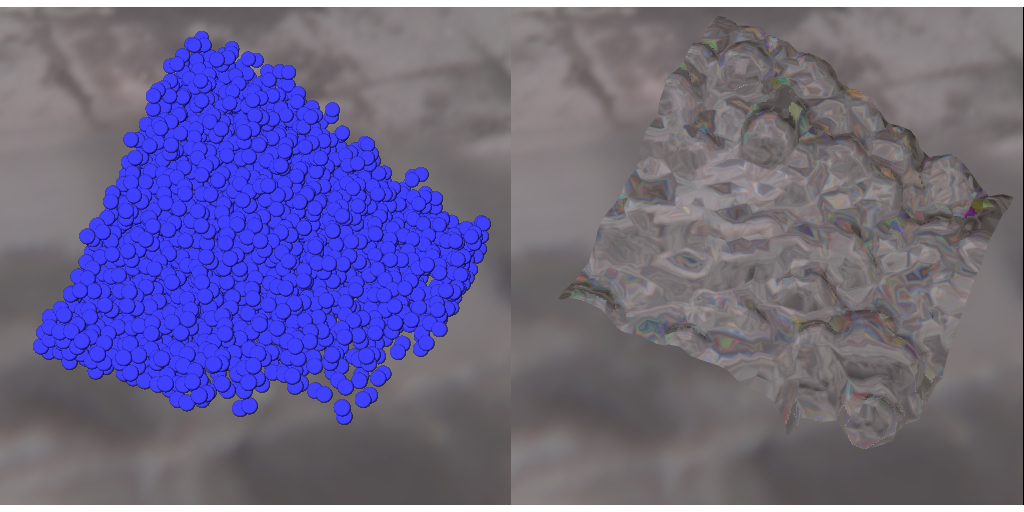
\includegraphics[width=0.9\textwidth]{figs/sph-plot.png}
  \end{center}
\end{frame}



\begin{frame}
  \frametitle{Pondering particles}
  
  \begin{itemize}
  \item Where do particles ``live'' (esp.~in distributed memory)?
    \begin{itemize}
    \item Decompose in space?  By particle number?
    \item What about clumping?
    \end{itemize}
  \item How are long-range force computations organized?
  \item How are short-range force computations organized?
  \item How is force computation load balanced?
  \item What are the boundary conditions?
  \item How are potential singularities handled?
  \item What integrator is used?  What step control?
  \end{itemize}
\end{frame}


\begin{frame}
  \frametitle{External forces}

  Simplest case: no particle interactions.
  \begin{itemize}
    \item Embarrassingly parallel (like Monte Carlo)!
    \item Could just split particles evenly across processors
    \item Is it that easy?
      \begin{itemize}
      \item Maybe some trajectories need short time steps?
      \item Even with MC, load balance may not be entirely trivial.
      \end{itemize}
  \end{itemize}
\end{frame}


\begin{frame}
  \frametitle{Local forces}
  
  \begin{center}
    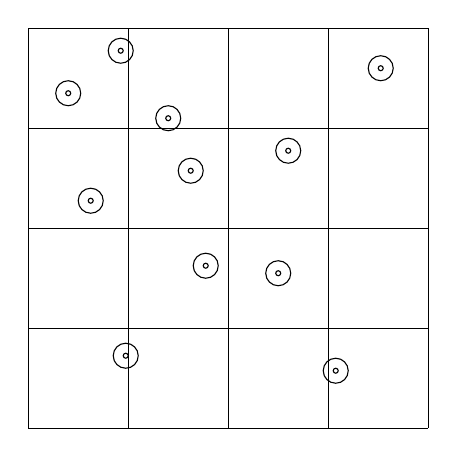
\begin{tikzpicture}[y=-1cm]

% objects at depth 50:
\draw[black] (2.44475,1.55575) circle (0.15875cm);
\draw[black] (2.44475,1.55575) circle (0.03175cm);
\draw[black] (1.778,2.0955) circle (0.15875cm);
\draw[black] (1.778,2.0955) circle (0.03175cm);
\draw[black] (3.33375,3.07975) circle (0.15875cm);
\draw[black] (3.33375,3.07975) circle (0.03175cm);
\draw[black] (3.048,2.413) circle (0.15875cm);
\draw[black] (3.048,2.413) circle (0.03175cm);
\draw[black] (2.06375,3.46075) circle (0.15875cm);
\draw[black] (2.06375,3.46075) circle (0.03175cm);
\draw[black] (3.52425,4.28625) circle (0.15875cm);
\draw[black] (3.52425,4.28625) circle (0.03175cm);
\draw[black] (4.445,4.3815) circle (0.15875cm);
\draw[black] (4.445,4.3815) circle (0.03175cm);
\draw[black] (4.572,2.82575) circle (0.15875cm);
\draw[black] (4.572,2.82575) circle (0.03175cm);
\draw[black] (5.74675,1.778) circle (0.15875cm);
\draw[black] (5.74675,1.778) circle (0.03175cm);
\draw[black] (2.50825,5.42925) circle (0.15875cm);
\draw[black] (2.50825,5.42925) circle (0.03175cm);
\draw[black] (5.17525,5.61975) circle (0.15875cm);
\draw[black] (5.17525,5.61975) circle (0.03175cm);
\draw[black] (1.27,1.27) -- (1.27,6.35);
\draw[black] (2.54,1.27) -- (2.54,6.35);
\draw[black] (3.81,1.27) -- (3.81,6.35);
\draw[black] (5.08,1.27) -- (5.08,6.35);
\draw[black] (6.35,1.27) -- (6.35,6.35);
\draw[black] (1.27,1.27) -- (6.35,1.27);
\draw[black] (1.27,2.54) -- (6.35,2.54);
\draw[black] (1.27,3.81) -- (6.35,3.81);
\draw[black] (1.27,5.08) -- (6.35,5.08);
\draw[black] (1.27,6.35) -- (6.35,6.35);

\end{tikzpicture}%

  \end{center}
  \begin{itemize}
  \item Simplest all-pairs check is $O(n^2)$ (expensive)
  \item Or only check close pairs (via binning, quadtrees?)
  \item Communication required for pairs checked
  \item Usual model: domain decomposition
  \end{itemize}

\end{frame}


\begin{frame}
  \frametitle{Local forces: Communication}

  \begin{center}
    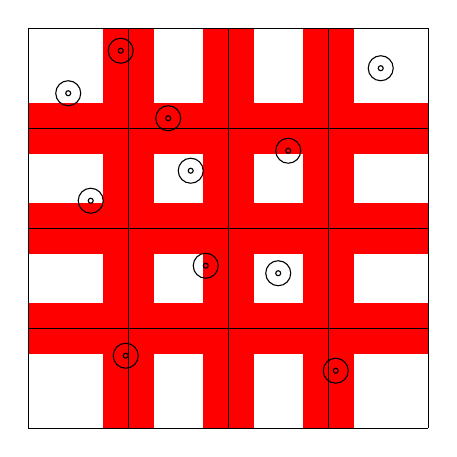
\begin{tikzpicture}[y=-1cm]

% objects at depth 60:
\filldraw[red] (2.2225,1.27) rectangle (2.8575,6.35);
\filldraw[red] (3.4925,1.27) rectangle (4.1275,6.35);
\filldraw[red] (4.7625,1.27) rectangle (5.3975,6.35);
\filldraw[red] (1.27,5.3975) rectangle (6.35,4.7625);
\filldraw[red] (1.27,4.1275) rectangle (6.35,3.4925);
\filldraw[red] (1.27,2.8575) rectangle (6.35,2.2225);

% objects at depth 50:
\draw[black] (2.44475,1.55575) circle (0.15875cm);
\draw[black] (2.44475,1.55575) circle (0.03175cm);
\draw[black] (1.778,2.0955) circle (0.15875cm);
\draw[black] (1.778,2.0955) circle (0.03175cm);
\draw[black] (3.33375,3.07975) circle (0.15875cm);
\draw[black] (3.33375,3.07975) circle (0.03175cm);
\draw[black] (3.048,2.413) circle (0.15875cm);
\draw[black] (3.048,2.413) circle (0.03175cm);
\draw[black] (2.06375,3.46075) circle (0.15875cm);
\draw[black] (2.06375,3.46075) circle (0.03175cm);
\draw[black] (3.52425,4.28625) circle (0.15875cm);
\draw[black] (3.52425,4.28625) circle (0.03175cm);
\draw[black] (4.445,4.3815) circle (0.15875cm);
\draw[black] (4.445,4.3815) circle (0.03175cm);
\draw[black] (4.572,2.82575) circle (0.15875cm);
\draw[black] (4.572,2.82575) circle (0.03175cm);
\draw[black] (5.74675,1.778) circle (0.15875cm);
\draw[black] (5.74675,1.778) circle (0.03175cm);
\draw[black] (2.50825,5.42925) circle (0.15875cm);
\draw[black] (2.50825,5.42925) circle (0.03175cm);
\draw[black] (5.17525,5.61975) circle (0.15875cm);
\draw[black] (5.17525,5.61975) circle (0.03175cm);
\draw[black] (1.27,1.27) -- (1.27,6.35);
\draw[black] (2.54,1.27) -- (2.54,6.35);
\draw[black] (3.81,1.27) -- (3.81,6.35);
\draw[black] (5.08,1.27) -- (5.08,6.35);
\draw[black] (6.35,1.27) -- (6.35,6.35);
\draw[black] (1.27,1.27) -- (6.35,1.27);
\draw[black] (1.27,2.54) -- (6.35,2.54);
\draw[black] (1.27,3.81) -- (6.35,3.81);
\draw[black] (1.27,5.08) -- (6.35,5.08);
\draw[black] (1.27,6.35) -- (6.35,6.35);

\end{tikzpicture}%

  \end{center}

  Minimize communication:
  \begin{itemize}
  \item Send particles that might affect a neighbor ``soon''
  \item Trade extra computation against communication
  \item Want low surface area-to-volume ratios on domains
  \end{itemize}
  
\end{frame}



\begin{frame}
  \frametitle{Local forces: Load balance}

  \begin{center}
    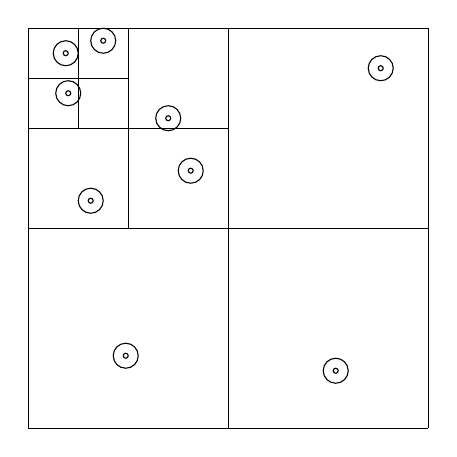
\begin{tikzpicture}[y=-1cm]

% objects at depth 50:
\draw[black] (1.778,2.0955) circle (0.15875cm);
\draw[black] (1.778,2.0955) circle (0.03175cm);
\draw[black] (3.33375,3.07975) circle (0.15875cm);
\draw[black] (3.33375,3.07975) circle (0.03175cm);
\draw[black] (3.048,2.413) circle (0.15875cm);
\draw[black] (3.048,2.413) circle (0.03175cm);
\draw[black] (2.06375,3.46075) circle (0.15875cm);
\draw[black] (2.06375,3.46075) circle (0.03175cm);
\draw[black] (5.74675,1.778) circle (0.15875cm);
\draw[black] (5.74675,1.778) circle (0.03175cm);
\draw[black] (2.50825,5.42925) circle (0.15875cm);
\draw[black] (2.50825,5.42925) circle (0.03175cm);
\draw[black] (5.17525,5.61975) circle (0.15875cm);
\draw[black] (5.17525,5.61975) circle (0.03175cm);
\draw[black] (1.74625,1.5875) circle (0.15875cm);
\draw[black] (1.74625,1.5875) circle (0.03175cm);
\draw[black] (2.2225,1.42875) circle (0.15875cm);
\draw[black] (2.2225,1.42875) circle (0.03175cm);
\draw[black] (1.27,1.27) -- (1.27,6.35);
\draw[black] (2.54,1.27) -- (2.54,3.81);
\draw[black] (3.81,1.27) -- (3.81,6.35);
\draw[black] (6.35,1.27) -- (6.35,6.35);
\draw[black] (1.27,1.27) -- (6.35,1.27);
\draw[black] (1.27,2.54) -- (3.81,2.54);
\draw[black] (1.27,3.81) -- (6.35,3.81);
\draw[black] (1.27,6.35) -- (6.35,6.35);
\draw[black] (1.27,1.905) -- (2.54,1.905);
\draw[black] (1.905,1.27) -- (1.905,2.54);

\end{tikzpicture}%

  \end{center}

  \begin{itemize}
  \item Are particles evenly distributed?
  \item Do particles remain evenly distributed?
  \item Can divide space unevenly (e.g.~quadtree/octtree)
  \end{itemize}
  
\end{frame}


\begin{frame}
  \frametitle{Far-field forces}

  \begin{center}
    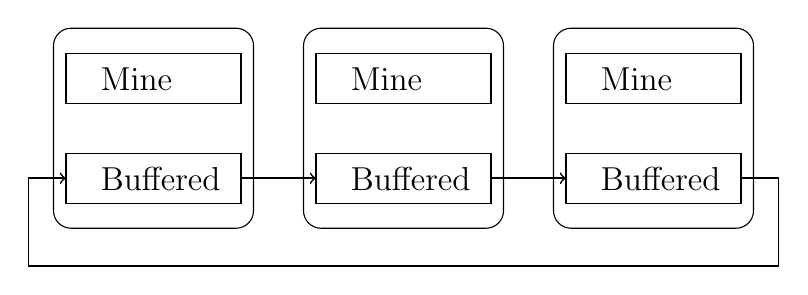
\begin{tikzpicture}[y=-1cm]

% objects at depth 50:
\draw[rounded corners=6.3bp,black] (5.08,5.08) rectangle (2.54,2.54);
\draw[black] (2.69875,2.8575) rectangle (4.92125,3.4925);
\draw[black] (2.69875,4.1275) rectangle (4.92125,4.7625);
\path (3.01625,3.33375) node[text=black,anchor=base west] {\large{}Mine};
\path (3.01625,4.60375) node[text=black,anchor=base west] {\large{}Buffered};
\draw[rounded corners=6.3bp,black] (8.255,5.08) rectangle (5.715,2.54);
\draw[black] (5.87375,2.8575) rectangle (8.09625,3.4925);
\draw[black] (5.87375,4.1275) rectangle (8.09625,4.7625);
\path (6.19125,3.33375) node[text=black,anchor=base west] {\large{}Mine};
\path (6.19125,4.60375) node[text=black,anchor=base west] {\large{}Buffered};
\draw[rounded corners=6.3bp,black] (11.43,5.08) rectangle (8.89,2.54);
\draw[black] (9.04875,2.8575) rectangle (11.27125,3.4925);
\draw[black] (9.04875,4.1275) rectangle (11.27125,4.7625);
\path (9.36625,3.33375) node[text=black,anchor=base west] {\large{}Mine};
\path (9.36625,4.60375) node[text=black,anchor=base west] {\large{}Buffered};
\draw[->,semithick,black] (4.92125,4.445) -- (5.87375,4.445);
\draw[->,semithick,black] (8.09625,4.445) -- (9.04875,4.445);
\draw[->,semithick,black] (11.27125,4.445) -- (11.7475,4.445) -- (11.7475,5.55625) -- (2.2225,5.55625) -- (2.2225,4.445) -- (2.69875,4.445);

\end{tikzpicture}%

  \end{center}

  \begin{itemize}
  \item Every particle affects every other particle
  \item All-to-all communication required
    \begin{itemize}
    \item Overlap communication with computation
    \item Poor memory scaling if everyone keeps everything!
    \end{itemize}
  \item Idea: pass particles in a round-robin manner
  \end{itemize}
\end{frame}


\begin{frame}[fragile]
  \frametitle{Passing particles for far-field forces}

  \begin{center}
    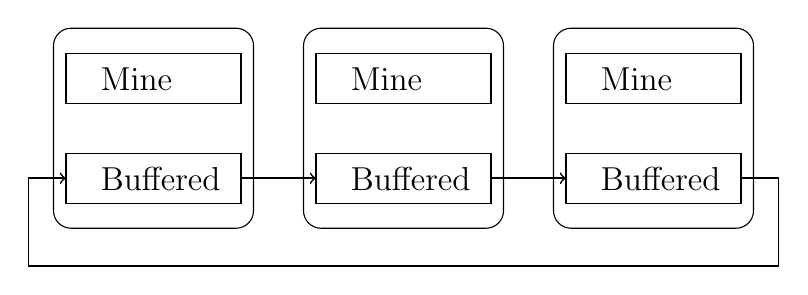
\begin{tikzpicture}[y=-1cm]

% objects at depth 50:
\draw[rounded corners=6.3bp,black] (5.08,5.08) rectangle (2.54,2.54);
\draw[black] (2.69875,2.8575) rectangle (4.92125,3.4925);
\draw[black] (2.69875,4.1275) rectangle (4.92125,4.7625);
\path (3.01625,3.33375) node[text=black,anchor=base west] {\large{}Mine};
\path (3.01625,4.60375) node[text=black,anchor=base west] {\large{}Buffered};
\draw[rounded corners=6.3bp,black] (8.255,5.08) rectangle (5.715,2.54);
\draw[black] (5.87375,2.8575) rectangle (8.09625,3.4925);
\draw[black] (5.87375,4.1275) rectangle (8.09625,4.7625);
\path (6.19125,3.33375) node[text=black,anchor=base west] {\large{}Mine};
\path (6.19125,4.60375) node[text=black,anchor=base west] {\large{}Buffered};
\draw[rounded corners=6.3bp,black] (11.43,5.08) rectangle (8.89,2.54);
\draw[black] (9.04875,2.8575) rectangle (11.27125,3.4925);
\draw[black] (9.04875,4.1275) rectangle (11.27125,4.7625);
\path (9.36625,3.33375) node[text=black,anchor=base west] {\large{}Mine};
\path (9.36625,4.60375) node[text=black,anchor=base west] {\large{}Buffered};
\draw[->,semithick,black] (4.92125,4.445) -- (5.87375,4.445);
\draw[->,semithick,black] (8.09625,4.445) -- (9.04875,4.445);
\draw[->,semithick,black] (11.27125,4.445) -- (11.7475,4.445) -- (11.7475,5.55625) -- (2.2225,5.55625) -- (2.2225,4.445) -- (2.69875,4.445);

\end{tikzpicture}%

  \end{center}

\begin{verbatim}
copy local particles to current buf
for phase = 1:p
  send current buf to rank+1 (mod p)
  recv next buf from rank-1 (mod p) 
  interact local particles with current buf
  swap current buf with next buf
end
\end{verbatim}
\end{frame}



\begin{frame}
  \frametitle{Passing particles for far-field forces}

  Suppose $n = N/p$ particles in buffer.  At each phase
  \begin{align*}
    t_{\mathrm{comm}} & \approx \alpha + \beta n \\
    t_{\mathrm{comp}} & \approx \gamma n^2
  \end{align*}
  So we can mask communication with computation if
  \[
  n \geq
    \frac{1}{2\gamma} \left( \beta + \sqrt{\beta^2 + 4 \alpha \gamma} \right)
    > \frac{\beta}{\gamma}
  \]

  \vspace{4mm}
  More efficient serial code \\
  $\implies$ larger $n$ needed to mask communication! \\
  $\implies$ worse speed-up as $p$ gets larger (fixed $N$) \\
  but scaled speed-up ($n$ fixed) remains unchanged.

  \vspace{4mm}
  This analysis neglects overhead term in LogP.
  
\end{frame}


\begin{frame}
  \frametitle{Far-field forces: particle-mesh methods}

  Consider $r^{-2}$ electrostatic potential interaction
  \begin{itemize}
  \item Enough charges looks like a continuum!
  \item Poisson equation maps charge distribution to potential
  \item Use fast Poisson solvers for regular grids (FFT, multigrid)
  \item Approximation depends on mesh and particle density
  \item Can clean up leading part of approximation error
  \end{itemize}

\end{frame}


\begin{frame}
  \frametitle{Far-field forces: particle-mesh methods}

  \begin{center}
    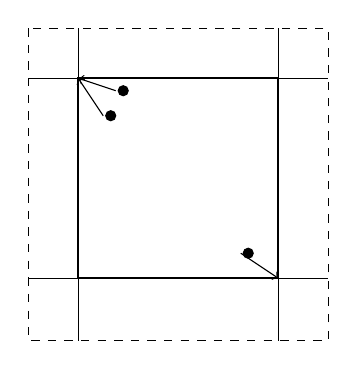
\begin{tikzpicture}[y=-1cm]

% objects at depth 50:
\filldraw[black] (4.3815,3.96875) circle (0.0635cm);
\filldraw[black] (5.969,6.0325) circle (0.0635cm);
\filldraw[black] (4.22275,4.28625) circle (0.0635cm);
\draw[black] (3.81,3.175) -- (3.81,7.14375);
\draw[black] (6.35,3.175) -- (6.35,7.14375);
\draw[black] (3.175,6.35) -- (6.985,6.35);
\draw[->,black] (4.1275,4.28625) -- (3.81,3.81);
\draw[semithick,black] (3.81,3.81) rectangle (6.35,6.35);
\draw[black] (3.175,3.81) -- (6.985,3.81);
\draw[->,black] (4.28625,3.96875) -- (3.81,3.81);
\draw[->,black] (5.87375,6.0325) -- (6.35,6.35);
\draw[dashed,black] (3.175,3.175) rectangle (6.985,7.14375);

\end{tikzpicture}%

  \end{center}
  
  \begin{itemize}
  \item Map particles to mesh points (multiple strategies)
  \item Solve potential PDE on mesh
  \item Interpolate potential to particles
  \item Add correction term -- acts like local force
  \end{itemize}

\end{frame}


\begin{frame}
  \frametitle{Far-field forces: tree methods}

  \begin{center}
    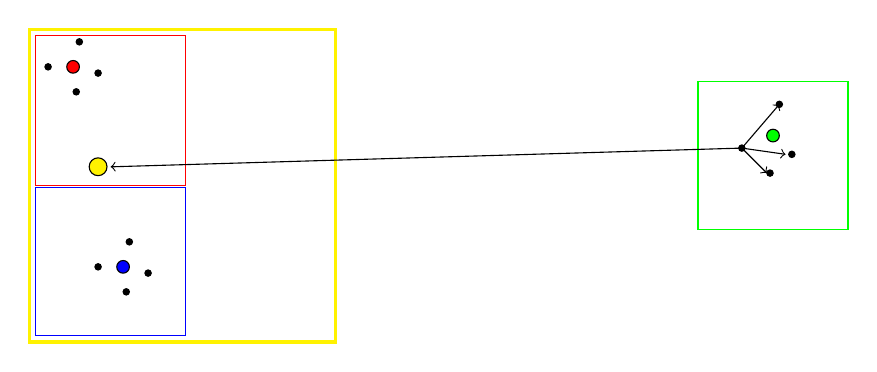
\begin{tikzpicture}[y=-1cm,scale=0.5]

% objects at depth 50:
\filldraw[black] (2.30293,1.42875) circle (0.08043cm);
\filldraw[black] (2.8575,0.9525) circle (0.08043cm);
\filldraw[black] (2.38125,0.15875) circle (0.08043cm);
\filldraw[black] (1.5875,0.79375) circle (0.08043cm);
\path[draw=black,fill=red] (2.2225,0.79375) circle (0.16087cm);
\filldraw[black] (3.57293,6.50875) circle (0.08043cm);
\filldraw[black] (4.1275,6.0325) circle (0.08043cm);
\filldraw[black] (3.65125,5.23875) circle (0.08043cm);
\filldraw[black] (2.8575,5.87375) circle (0.08043cm);
\path[draw=black,fill=blue] (3.4925,5.87375) circle (0.16087cm);
\path[draw=black,fill=yellow] (2.8575,3.33163) circle (0.22648cm);
\filldraw[black] (19.92418,3.4925) circle (0.08043cm);
\filldraw[black] (20.47875,3.01625) circle (0.08043cm);
\filldraw[black] (19.20875,2.8575) circle (0.08043cm);
\filldraw[black] (20.16125,1.74625) circle (0.08043cm);
\path[draw=black,fill=green] (20.00038,2.54) circle (0.16087cm);
\draw[semithick,red] (1.27,0) rectangle (5.08,3.81);
\draw[semithick,blue] (1.27,3.8608) rectangle (5.08,7.62);
\draw[very thick,yellow] (1.11125,-0.15875) rectangle (8.89,7.77875);
\draw[semithick,green] (18.0975,1.16205) rectangle (21.9075,4.92125);
\draw[arrows=-to,black] (19.20875,2.8575) -- (3.175,3.33375);
\draw[arrows=-to,black] (19.20875,2.8575) -- (20.16125,1.74625);
\draw[arrows=-to,black] (19.20875,2.8575) -- (20.32,3.01625);
\draw[arrows=-to,black] (19.20875,2.8575) -- (19.84375,3.4925);

\end{tikzpicture}%

  \end{center}
  \begin{itemize}
  \item Distance simplifies things
    \begin{itemize}
    \item Andromeda looks like a point mass from here?
    \end{itemize}
  \item Build a tree, approximating descendants at each node
  \item Several variants: Barnes-Hut, FMM, Anderson's method
  \item More on this later in the semester
  \end{itemize}
\end{frame}


\begin{frame}
  \frametitle{Summary of particle example}

  \begin{itemize}
  \item Model: Continuous motion of particles
    \begin{itemize}
    \item Could be electrons, cars, whatever...
    \end{itemize}
  \item Step through discretized time
  \item Local interactions
    \begin{itemize}
    \item Relatively cheap
    \item Load balance a pain
    \end{itemize}
  \item All-pairs interactions
    \begin{itemize}
    \item Obvious algorithm is expensive ($O(n^2)$)
    \item Particle-mesh and tree-based algorithms help
    \end{itemize}
  \end{itemize}

  An important special case of lumped/ODE models.
\end{frame}

\end{document}
